In this chapter, we are going to demostrate the experimental Work done on the laboratory and the preparation of the setup of the quarter car model with the passive suspension system then to be transformed and compared to the active suspension system.
\section{Physical Model Parameters Determination}
  

According to the chapter 7 VEHICLE RIDE CHARACTERISTICS \cite{wong2001theory},the natural frequencies of the unsprung 
mass (tire/wheel assembly) is around 10 Hz and the sprung mass (Vehicle Body) is aroung the 1 Hz.
So in our study, we tried to be around this range of values.
To determine specifically the values of the suspension parameteres to conserve these values, get the governing equations, as shown:

\begin{equation}
    f_{n-s} =\frac{1}{2\pi} \sqrt{\frac{\frac{k k_{t}}{k+k_{t}} }{M} }
    \label{eqn:3.1}
\end{equation}

\begin{equation}
    f_{n-us} =\frac{1}{2\pi} \sqrt{\frac{k k_{t}}{m }}
    \label{eqn:3.2}
\end{equation}
where: 

\begin{itemize}
    \item \( f_{n-s} \): is the sprung mass natural frequency
    \item \( f_{n-{us}} \): is the unsprung mass natural frequency
    \item \( k \): is the spring stiffness
    \item \( k_{t} \): is the tire stiffness
    \item \( M \): is the sprung mass
    \item \( m \): is the unsprung mass
\end{itemize}

\newpage
Therefore,the parameters values which are selected shown in the following table:

\begin{table}[h]
    \centering
    \caption{Physical Model Parameters}
    \begin{tabular}{lccc}

        \hline
        \textbf{Parameter} & \textbf{Symbol} & \textbf{Value}  & \textbf{Unit}  \\
        \hline

        Sprung mass & \( M\)& 30 & kg\\
        Unsprung mass & \( m \)& 13 & kg\\
        Spring stiffness & \( k \)& 6921 & N/m\\ 
        Tire stiffness & \( k_{t} \)& 81000 & N/m\\
        Damper average damping coefficient & \( b_{s} \)& 900 & N s/m\\
        Tire damping coefficient & \( b_{tr} \)& 0 & N s/m\\

        \hline
        \label{table:Parameter}
    \end{tabular}
\end{table}
\begin{figure}[H]
    \centering
    \includegraphics[width=0.45\textwidth]{layout labeled.png}
    \caption{Passive Physical Model Setup}
    \label{fig:Passive layout}
\end{figure}
The natural frequencies, according to the parameters demostrated in table \ref{table:Parameter} and by using the equations  \ref{eqn:3.1} and \ref{eqn:3.2}, are \( f_{n-s} \)  approximately equals to 2.33 Hz and \( f_{n-{us}} \)  approximately equals to 13 Hz.






\newpage
\section{Road Excitation}
To this point, our physical model is ready to behave with the road irregularities.
The road excitation is illustrated in the following figure:
\begin{figure}[H]
    \centering
    \includegraphics[width=0.8\textwidth]{Excitation mechanism.png}
    \caption{Road Excitation Mechanism}
    \label{fig:Excitation mechanism}
\end{figure}
As shown in the above Figure \ref{fig:Excitation mechanism}, the motion is given from a three-phase electric motor with chain-Sprocket mechanism which rotates the rotating Disc equipped with a V-slot that allows changing the crank length, by changing the eccentricity, of the slider-crank mechanism, consequencly change the road excitation amplitude. The following two figures will demostrate the chain-Sprocket mechanism Figure \ref{fig:chain-Sprocket mechanism} and the slider-crank mechanism Figure \ref{fig:Slider-Crank Mechanism}.
\begin{figure}[H]
    \centering
    \includegraphics[width=0.6\linewidth]{Chain-Sprocket mechanism.png}
    \caption{Chain-Sprocket Mechanism}
    \label{fig:chain-Sprocket mechanism}
\end{figure}

\begin{figure}[H]
    \centering
    \includegraphics[width=0.3\linewidth]{Slider Crank Mechanism.png}
    \caption{Slider-Crank Mechanism}
    \label{fig:Slider-Crank Mechanism}
\end{figure}

The three-phase electric motor is driven by an inverter shown in figure \ref{fig:Inverter} .  
\begin{figure}[H]
    \centering
    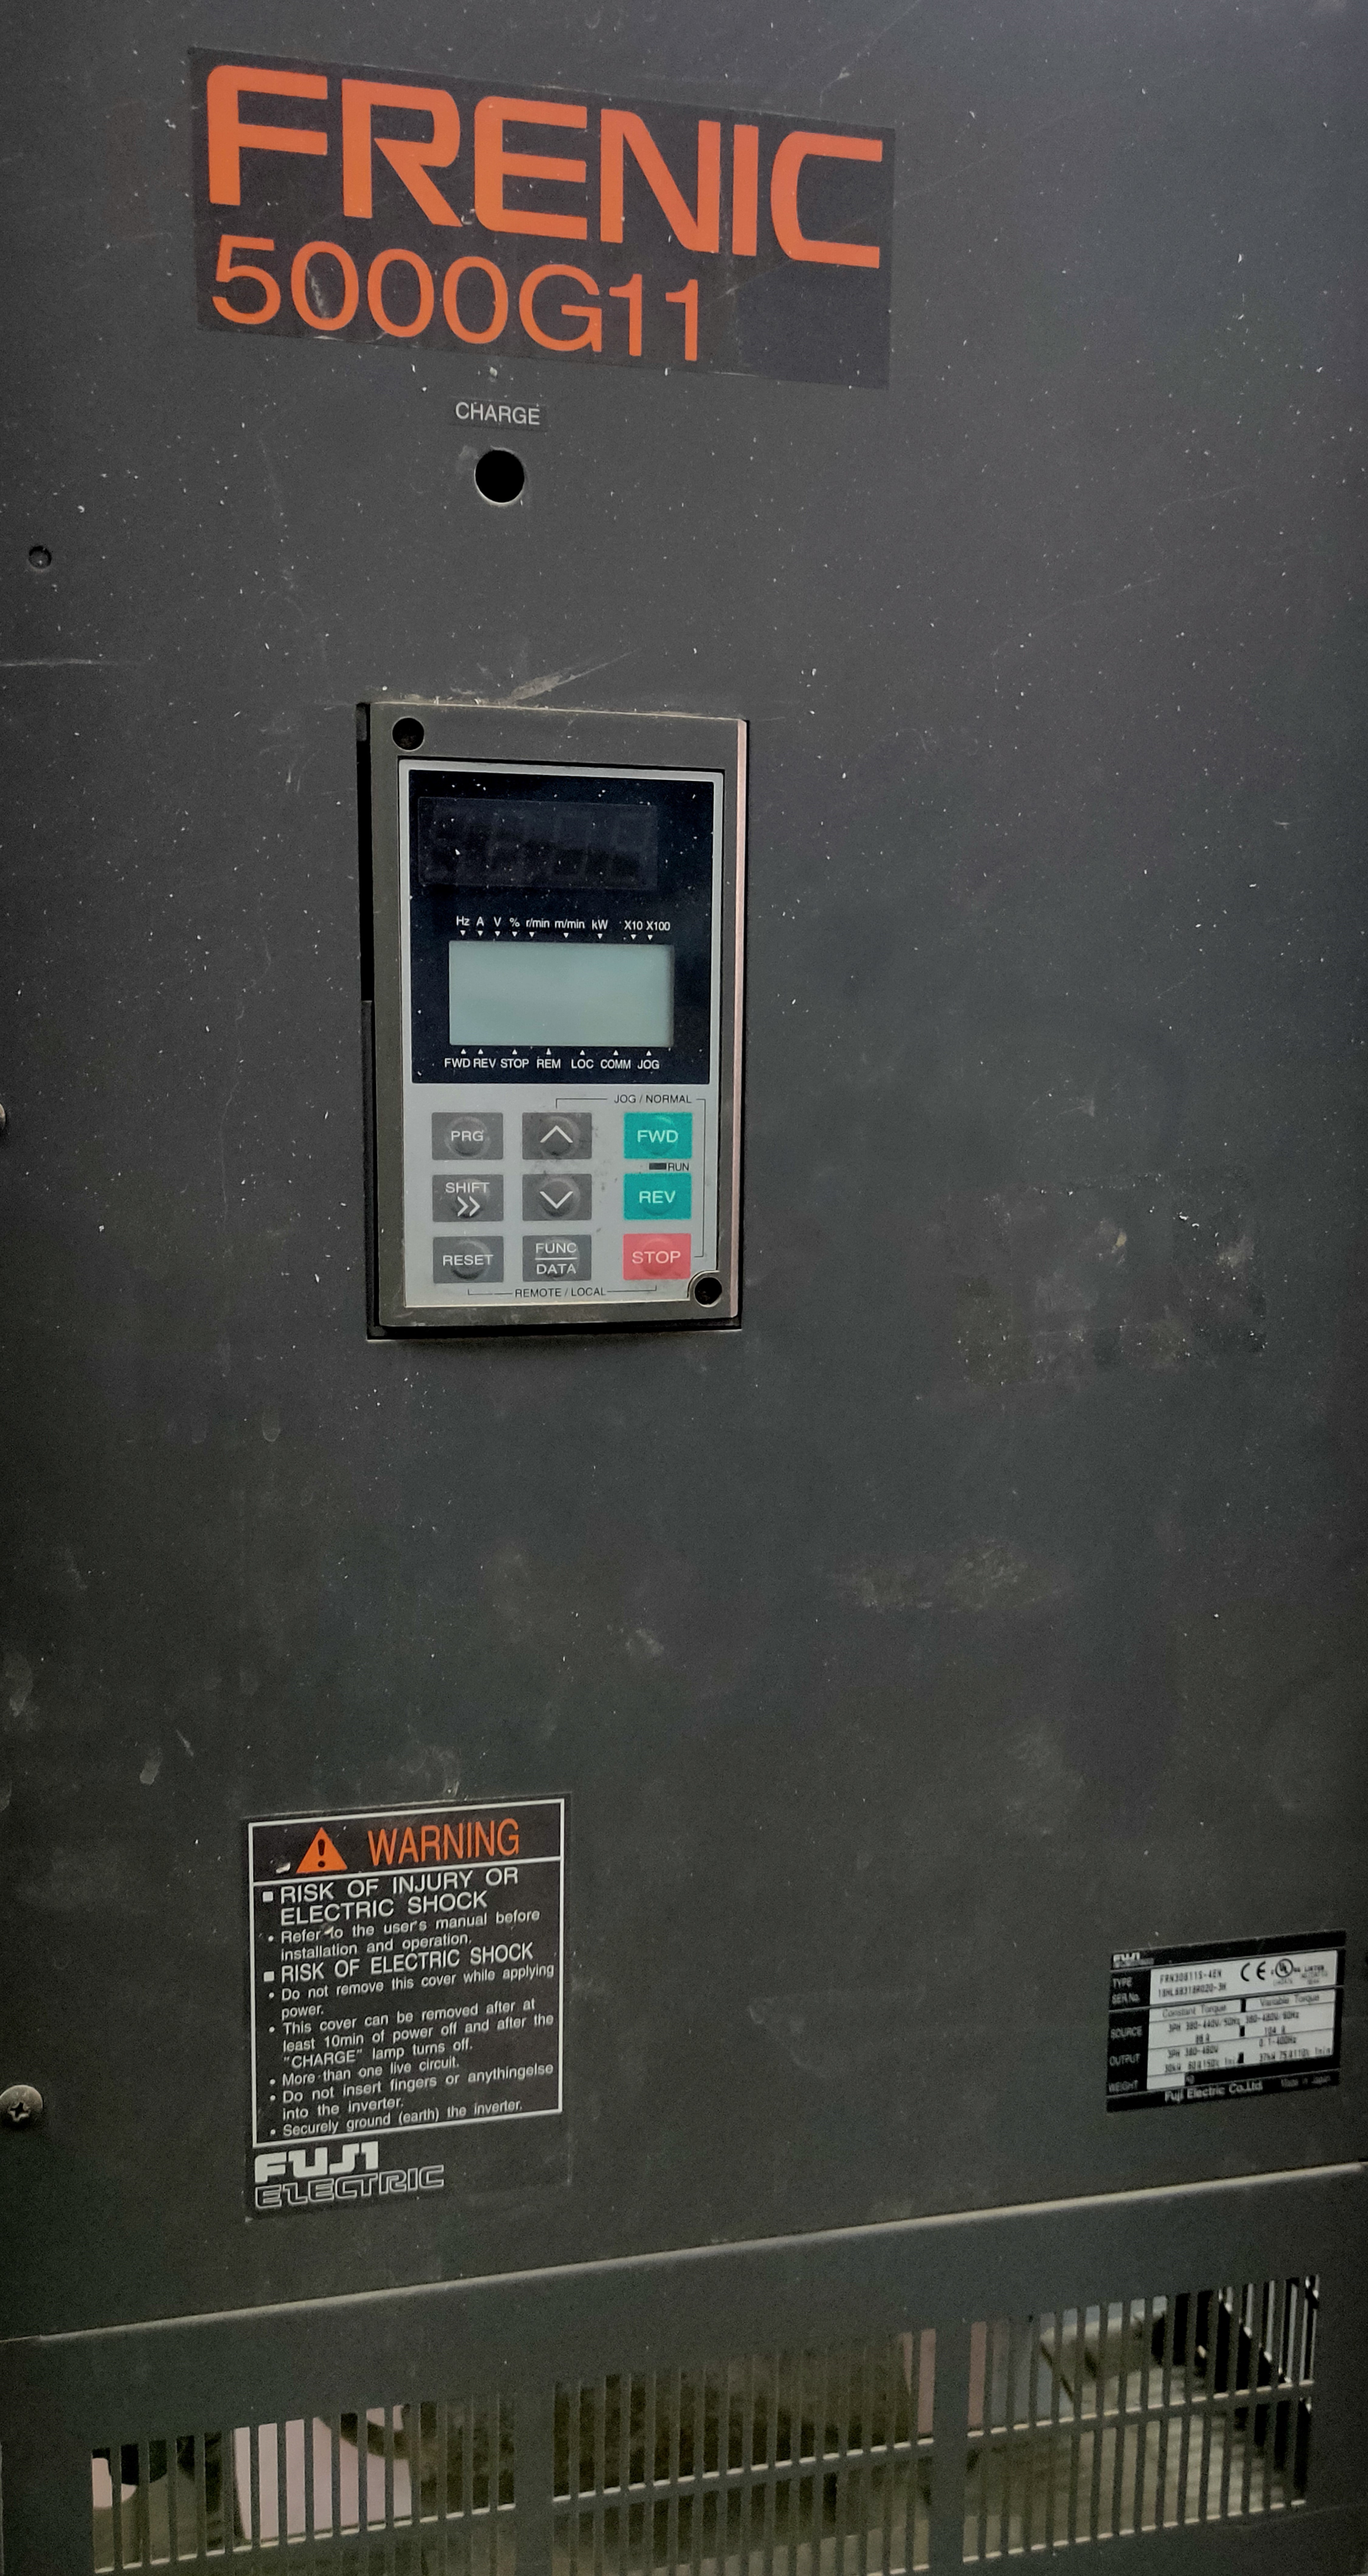
\includegraphics[width=0.2\textwidth]{Inverter.jpg}
    \caption{Variable Frequency Drive (VFD)}
    \label{fig:Inverter}
    
\end{figure}
Inverters play a crucial role in the control and operation of three-phase electric motors. An inverter, also known as a Variable Frequency Drive (VFD), converts the fixed-frequency AC power supply into a variable-frequency output. This conversion allows precise control over the motor’s speed and torque. By adjusting the frequency and voltage supplied to the motor, the inverter can smoothly start and stop the motor, reducing mechanical stress and extending the lifespan of both the motor and the associated machinery. Additionally, inverters improve energy efficiency by matching the motor’s speed to the actual demand, leading to significant energy savings, especially in applications with varying load requirements. The flexibility and control provided by inverters are essential in modern industrial processes, making them indispensable in achieving optimized performance and enhanced operational efficiency of three-phase electric motors.
\newpage

\section{Data Reception}
Once the physical model is running, we want to get the data quantitatively to be analyzed in the following chapters, this data is the displacement done caused by the road excitation either the sprung and the unsprung masses.

\subsubsection{Industrial Displacement Sensors}

Industrial Linear Potentiometers and LVDT were considered as an option but upon checking the available market prices for the required specifications, it concluded that such an approach is out of the budget limit of the project.

\subsection{Displacement Sensor Design}

Despite the many possibilities presented by contemporary sensor technologies; each solution encountered its own set of limitations. Issues such as sensitivity to external factors, suboptimal precision, and challenges related to market state and budget, evident through the extensive testing and experimentation phase. It became increasingly apparent that a tailored approach was necessary to address the demands of our application.

In response to these challenges, a decisive solution emerged: the design and implementation of a mechanical displacement sensor. This approach draws inspiration from the fundamental principles of mechanical engineering and the common industrial sensors, to overcome the shortcomings encountered during the exhaustive sensor trials.

\subsubsection{Working Principle}
The sensor design is rendered as shown in figure \ref{fig:sensor renderings}.
Reliance was placed onto converting the semi-vertical movement of the vehicle while traveling over an undulating surface into a rotary movement via a rack and pinion. The rack is fixed to the vehicle and when the vehicle traveling over an undulating surface, the rack is moved and thus vertical movement is transferred via the pinion to rotary movement, and then through a connection between the pinion and the potentiometer, the value of the change in resistance inside the potentiometer is an indication to certain displacement.

It is important to note that the rack is connected to a ball joint to allow slight misalignment as the sensor extends and retracts.
This is necessary because the actual movement of the vehicle, when climbing a bump, follows a curved path rather than a strictly vertical one.
The choice of a helical rack and pinion was made to increase contact area, reduce noise, and minimize impact.
\begin{table}[H]
    \centering
    \caption{Sensor Specifications.}
    \begin{tabular}{ l|l }
        \hline
        Stroke                             & 100 [mm]             \\
        Input Voltage                      & 3.3 - 5 [V]          \\
        Rack and Pinion Type               & Helical (30$^o$ deg) \\
        Accuracy                           & 0.01 [mm]            \\
        Max Deviation                      & 5\%                  \\
        Total Length (Fully Extended)      & 320 [mm]             \\
        Eye-to-eye Length (Fully Extended) & 305.2 [mm]           \\
        Total Cost                         & 390 [L.E.]           \\
        \hline
    \end{tabular}
    \label{table:sensor}
\end{table}

\begin{figure}[H]
    \centering
    \begin{subfigure}{\textwidth}
        \centering
        \includegraphics[width=0.5\textwidth]{Assembly.png}
    \end{subfigure}
    \begin{subfigure}{\textwidth}
        \centering
        \includegraphics[width=0.5\textwidth]{Assemblysec.png}
    \end{subfigure}
    \caption{Renderings of the designed displacement sensor, showing potentiometer and helical gear and rack as well as ball joints.}
    \label{fig:sensor renderings}
\end{figure}

The sensor was designed to meet all the requirements for a displacement sensor, and the displacement data acquired was sufficient to be used in deriving the acceleration of both the sprung and unsprung masses, making it suitable for future active suspension controller design.
With the sampling rate being dependent on the controller processing speed, this showed superior advantage over the module-based sensors used previously, which rely on the on-board processing to produce the data.

The noise generated by the sensor was at minimum-to-none levels and the sensor was calibrated to a precision micrometer with a deviation of 0.01 mm from the true readings at extremes.

The cost of the sensor, although pricier than electronic sensors used above, was much cheaper than industrial alternatives, with almost the same performance at \underline{one tenth of the price}. However, industrial sensors provide superior environmental resistance, which isn't particularly available in case of this sensor.
\begin{figure}[H]
    \centering
    \includegraphics[width=0.6\linewidth]{calb[1].pdf}
    \caption{Diplacement sensor calibration. \cite{malaric2011instrumentation}}
\end{figure}
\newpage
\subsection{Displacement Sensors Fixation}
Three displacement sensors were manufactured and fixed to receive the road input displacement, the unsprung mass displacement and the sprung mass displacement.
The sensors fixation to the physical model is illustrated in the following figure.
\begin{figure}[H]
    \centering
    \includegraphics[width=0.9\textwidth]{Sensors Fixation.jpg}
    \caption{Displacement Sensors Setup}
    \label{fig:Sensors Fixation}
    
\end{figure}

\newpage
\section{Active Physical Model Setup}
As discussed above, we going to compare between the conventional passive suspension system with the modified active suspension system. So, the comparison to be fair we going to conserve the natural frequencied as possible because the masses will differ as we add the active component that is the linear actuator. The schematic diagram of the system will be shown in the following figure\ref{fig:Active schematic diagram}:
\begin{figure}[H]
    \centering
    \includegraphics[width=0.4\textwidth]{Active schematic diagram.png}
    \caption{Schematic Diagram of the Modified Active Suspension System \cite{wong2001theory}}
    \label{fig:Active schematic diagram}
    
\end{figure}
The setup of the modified Active suspension System is shown in the following figure:

\begin{figure}[H]
    \centering
    \includegraphics[width=0.9\textwidth]{Active Setup.png}
    \caption{Setup of the Modified Active Suspension System }
    \label{fig:Active schematic diagram}
    
\end{figure}
\newpage
The parameters of the modified system is listed in the table below.
\begin{table}[h]
    \centering
    \caption{Modified Physical Model Parameters}
    \begin{tabular}{lccc}

        \hline
        \textbf{Parameter} & \textbf{Symbol} & \textbf{Value}  & \textbf{Unit}  \\
        \hline

        Sprung mass & \( M \)& 34 & kg\\
        Unsprung mass & \( m \)& 11 & kg\\
        Spring stiffness & \( k \)& 6921 & N/m\\ 
        Tire stiffness & \( k_{t} \)& 81000 & N/m\\
        \hline
        \label{table:Parameter}
    \end{tabular}
\end{table}

Therefore, the natural frequencies will be calculated as previously mentioned and by using the equations \ref{eqn:3.1} and \ref{eqn:3.2},also expected that the values will change a little bit but are in the range are \( f_{n-s} \)  approximately equals to 2.2 Hz and \( f_{n-{us}} \)  approximately equals to 14 Hz.
\newpage
\section{Noise Rejection}
In the phase of the data reception by the displacement sensor, as shown in Figure \ref{fig:Displacement Sensor}, we faced that the data was distorted.
\begin{figure}[H]
    \centering
    \includegraphics[width=0.2\textwidth]{Sensor.png}
    \caption{Displacement Sensor}
    \label{fig:Displacement Sensor}
    
\end{figure}
After searching for the reasons of the data distortion to be mitigated, we find that this noise is known as Electromagnetic Interference (EMI) \cite{digimaxEMI}.
Electromagnetic noise, often referred to as electromagnetic interference (EMI), is a pervasive and troublesome issue in the world of electronic circuits and devices. It's a phenomenon that can wreak havoc on the performance and reliability of electronic systems, leading to malfunctions, data corruption, and even safety hazards in critical applications. Understanding electromagnetic noise is essential for engineers and designers striving to create robust and reliable electronic products\cite{fastercapitalEMNoise}.
EMI can be caused by a variety of factors, including:
\begin{itemize}
    \item Radio frequency (RF) emissions.
    \item Electrostatic discharge (ESD).
    \item Power surges.
    \item and Lightning strikes.
\end{itemize}
   RF emissions can come from various sources, including communication devices, radar systems, and navigation equipment. ESD, on the other hand, occurs when there is a sudden discharge of static electricity. Power surges can happen when there is a sudden increase in voltage, while lightning strikes can cause significant damage to electronic systems\cite{digimaxEMI} \cite{fastercapitalEMNoise}.
\newline
The data distorted is illustrated in the following figure.
\begin{figure}[H]
    \centering
    \includegraphics[width=0.7\textwidth]{Data distorted.jpg}
    \caption{Distorted data of the Displacement Sensor, data taken by BetterSerialPlotter sofware}
    \label{fig:Distorted data}
    
\end{figure}
One of the mitigation methods is grounding.
\newline
Grounding is the establishment of an electrically conductive path between an electrical or electronic element of a system and a reference point or plane referenced to ground and it can refer to an electrical connection made to Earth as well. 

To achieve the best possible ground include: 
\begin{itemize}
    \item Keep leads away from internal circuits or other components to ground as short as possible to reduce inductance.
    \item Use multiple grounding points on a large ground plane for best results. 
    \item Try to isolate circuits from ground if ground loop voltages can’t be controlled any other way.
    \item Maintain separate grounds for analogue and digital circuits-- you can combine them later at a single point\cite{ttelectronicsEMI}.
\end{itemize}

The shield wire is connected to the ground which is shown in Figure \ref{fig:Signal and Shield Wires}
\begin{figure}[H]
    \centering
    \includegraphics[width=0.25\textwidth]{Shild wire.png}
    \caption{Signal and Shield Wires}
    \label{fig:Signal and Shield Wires}
    
\end{figure}
 After the grounding of the shield wire was done, the data is improved and the result is shown in the following figure:
 \begin{figure}[H]
    \centering
    \includegraphics[width=0.7\textwidth]{Improved data.jpg}
    \caption{Grounding Effect on the data}
    \label{fig:Grounding Effect}
    
\end{figure}
\newpage
Also the effect will be shown better in the following figure  that shows the signal before and after the grounding of the shield wire.
\begin{figure}[H]
    \centering
    \includegraphics[width=0.9\textwidth]{Comparison.png}
    \caption{Before and After Shield Wire Grounding}
    \label{fig:Comparison}
    
\end{figure}
\newpage
\section{Test-rig Modification and Additional Fixations}
\subsection{Test-rig Modification}
Test-rig was capable for one degree of freedom setup as shown in the figure \ref{fig:One Degree of freedom Test-rig Setup}. So, one task is set to modify the test-rig to be capable for two-degree of freedom with the required parts design and manufacture as shown in figure\ref{fig:Two-Degree of Freedom Test-rig Setup}.
\begin{figure}[H]
    \centering
    \includegraphics[width=0.2\textwidth]{Test rig(one degree).png}
    \caption{one degree of freedom Test-rig Setup}
    \label{fig:One Degree of freedom Test-rig Setup}
\end{figure}
\begin{figure}[H]
    \centering
    \includegraphics[width=0.2\textwidth]{passive layout.jpg}
    \caption{Two-Degree of Freedom Test-rig Setup}
    \label{fig:Two-Degree of Freedom Test-rig Setup}
\end{figure}
\newpage
\subsection{Additional Fixations and Extension Rods}
After Modified the test-rig to two-degree of freedom and finish the passive model phase, the test-rig is going to be modified to be capable for the Active physical model. The challenge faced is the actuator needs more vertical space; So, the rods going to be extended by the extention rods, shown in the following figure \ref{fig:Extension Rods} and its working drawing .
\begin{figure}[H]
    \centering
    \includegraphics[width=0.7\textwidth]{Extention Rods.png}
    \caption{Extension Rods}
    \label{fig:Extension Rods}
\end{figure}
\begin{figure}[H]
    \centering
    \includegraphics[width=0.9\textwidth]{ER Working Drawing.png}
    \caption{Extension Rod Working Drawing}
    \label{fig:Extension Rod Working Drawing}
\end{figure}
\newpage
Also, another problem is faced is the upper sway of the test-rig caused by the extention of its length. The solution was the fixation of the test-rig upper point to the wall to prevent the sway motion.
\newline
The following figure illustrate the fixation to the wall.  
\begin{figure}[H]
    \centering
    \includegraphics[width=0.7\textwidth]{Wall Fixation.jpg}
    \caption{Fixation to the wall}
    \label{fig:Fixation}
\end{figure}

\newpage
\section{Active Component of the System}
In this section we are going to identify the active component of the modified active suspension system, which is the linear actuator with its driver, also will show the required connections.

\subsection{Specifications of the Linear Actuator}
Linear motor (actuator) is the same as brushless AC motor. Instead of the permanent magnet pairs on the rotor, the linear motor rod consists of an array of magnets strips, as shown in figure \ref{fig:Actuator Construction} The windings are also along the force tube instead of being on the stator. 
\begin{figure}[H]
    \centering
    \includegraphics[width=0.5\textwidth]{Linear Actuator construction.png}
    \caption{Schematic representation of the Linear acturator \cite{nipponpulseLinearMotors}}
    \label{fig:Actuator Construction}
    
\end{figure}
The required motor will be with three-phase windings to be able to change the output force and direction.
\newline
The linear actuator is from Copley Motion Systems company\cite{copleymotion} with part number of XTB3810S-S-S05D, as shown the figure below.
\begin{figure}[H]
    \centering
    \includegraphics[width=0.9\textwidth]{Actuator Part no..png}
    \caption{XTB3810S-S-S05D Linear Actuator}
    \label{fig:Actuator}
    
\end{figure}
\newpage
\subsection{Specifications of the Linear Actuator Driver}
The linear actuator needs a driver to operate. The suitable driver that was used in the experiments is known with the model no. of Xenus XTL-230-36 shown below.
\begin{figure}[H]
    \centering
    \includegraphics[width=0.7\textwidth]{Driver Specs.jpg}
    \caption{Driver of the Linear Actuator}
    \label{fig:Driver}
    
\end{figure}

The driver dimensions are [in mm]: 192 x 142 x 65
\subsection{Installation of the Linear Actuator Driver}
The driver installation is illustrated in the following diagram.
\begin{figure}[H]
    \centering
    \includegraphics[width=0.8\textwidth]{Driver Installation.png}
    \caption{Driver of the Linear Actuator(From Data sheet)}
    \label{fig:Driver}
    
\end{figure}

\subsection{Actuator-Driver Connections Illustration}
\begin{figure}[H]
    \centering
    \includegraphics[width=0.99\textwidth]{driver lower wiring.png}
    \caption{Main Connections}
    \label{fig:Main Connections}
    
\end{figure}
\begin{figure}[H]
    \centering
    \includegraphics[width=0.99\textwidth]{Serial cable.png}
    \caption{Serial connection and motor feedback cable}
    \label{fig:Serial connection}
    
\end{figure}
\newpage
So, the connections are made, according to the data sheet,as shown in figures \ref{fig:Main Connections} and \ref{fig:Serial connection}, shown below.
\begin{figure}[H]
    \centering
    \includegraphics[width=0.99\textwidth]{Lower Driver connections.jpg}
    \caption{Motor main connections to the driver}
    \label{fig:Connections}
    
\end{figure}

\begin{figure}[H]
    \centering
    \includegraphics[width=0.99\textwidth]{Feedback and serial cable.jpg}
    \caption{Serial and motor feedback cables}
    \label{fig:serialConnections}
    
\end{figure}
\newpage
\subsection{Control Signals Connections}
The control signals that will be send from the controller connected to the control signals port and the pins used as shown in the following figure.

\begin{figure}[H]
    \centering
    \includegraphics[width=0.99\textwidth]{Control Signals.png}
    \caption{Control Signals Connections}
    \label{fig:Control Signals}
    
\end{figure}
Xenus has twelve digital inputs, eleven of which have programmable functions. Input [IN1] is dedicated to the drive Enable function. 
This is done to prevent accidental programming of the input in such a way that the controller could not shut it down.
Two types of RC filters are used: GP (general purpose) and HS (high speed). Input functions such as Pulse/Dir, CW/CCW, Quad A/B are 
wired to inputs having the HS filters, and inputs with the GP filters are used for general purpose logic functions, limit switches, and the 
motor temperature sensor. 
The digital pins [IN9] HS and [IN10] HS are used to be pulse and Direction signals respectively,shown in figure \ref{fig:Single-Ended Pulse and Direction}.

\begin{figure}[H]
    \centering
    \includegraphics[width=0.6\textwidth]{Pulse and Dir.png}
    \caption{Single-Ended Pulse and Direction}
    \label{fig:Single-Ended Pulse and Direction}
    
\end{figure}


